\usetikzlibrary{arrows, shadows, decorations.markings}
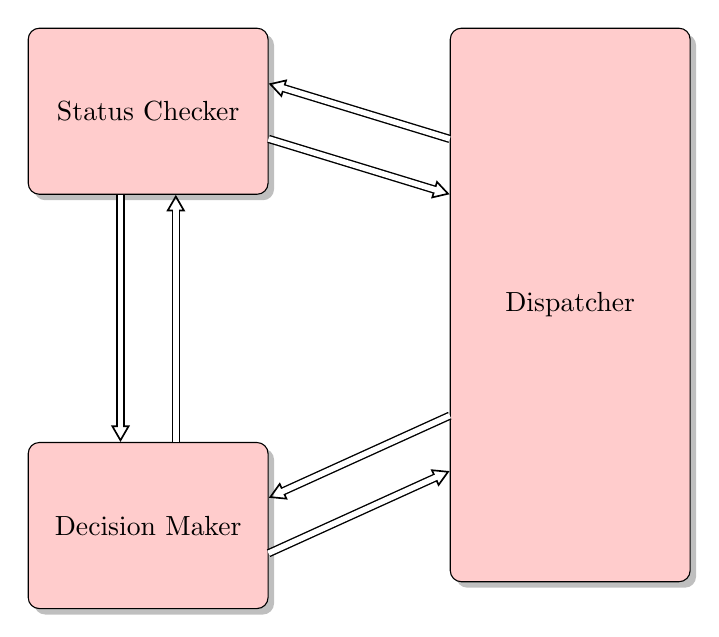
\begin{tikzpicture}
  \tikzstyle{vecArrow} = [thick, decoration={markings,mark=at position
	1 with {\arrow[semithick]{open triangle 60}}},
	double distance=1.4pt, shorten >= 5.5pt, preaction = {decorate},
	postaction = {draw,line width=2pt, white,shorten >= 4.5pt}
  ]
  \tikzstyle{component} = [draw,text centered,rounded corners,drop
  shadow,text width=8em,fill=red!20,minimum height=6em]
  \tikzstyle{dispatcher} = [component,minimum height=20em]

  % Define the layers to draw the diagram
  \pgfdeclarelayer{background}
  \pgfdeclarelayer{foreground}
  \pgfsetlayers{background,main,foreground}

  % Define distances for bordering
  \def\blockdist{2.3}
  \def\edgedist{2.5}

  \node[component](status-checker){Status Checker};
  \path (status-checker.north east)+(\blockdist,0) node[dispatcher, anchor=north west](dispatcher){Dispatcher};
  \path (status-checker.south)+(0,-4.2) node[component](decision-maker){Decision Maker};
  \draw[vecArrow] ([xshift=-10]status-checker.south) to ([xshift=-10]decision-maker.north);
  \draw[vecArrow] ([xshift=10]decision-maker.north) to ([xshift=10]status-checker.south);

  \def\composhift{50}
  \draw[vecArrow] ([yshift=-10]status-checker.east) to ([yshift=-10+\composhift]dispatcher.west);
  \draw[vecArrow] ([yshift=10+\composhift]dispatcher.west) to([yshift=10]status-checker.east);

  \draw[vecArrow] ([yshift=-10]decision-maker.east) to ([yshift=-10-\composhift]dispatcher.west);
  \draw[vecArrow] ([yshift=10-\composhift]dispatcher.west) to ([yshift=10]decision-maker.east) ;
\end{tikzpicture}
